% 교수님 설득용 브리프 (2026-10-13). tectonic -o docs/paper docs/paper/brief_prof.tex
\documentclass[10pt,a4paper]{article}
\usepackage{kotex}
\IfFontExistsTF{Noto Sans CJK KR}{\setmainhangulfont{Noto Sans CJK KR}}{\setmainhangulfont{Malgun Gothic}}
\usepackage[margin=18mm]{geometry}
\usepackage{amsmath,amssymb}
\usepackage{booktabs,array,enumitem}
\usepackage{graphicx}
\usepackage[colorlinks=true,linkcolor=blue,urlcolor=blue]{hyperref}
\usepackage{xcolor}
\newcommand{\method}{CCD}
\setlist{nosep}
\graphicspath{{./}}
\title{\vspace{-8mm}연구 브리프: FL$\to$FU 공격 부류의 정의와 학습 중 방어}
\author{(발표자)}
\date{2026-10-13}
\begin{document}
\maketitle
\vspace{-6mm}

\section{한 장 요약}
\begin{itemize}
\item \textbf{막으려는 것.} 특정 두 논문(FUBA, BadFU)이 아니라, \emph{연합학습(FL) 중에 심고 연합 언러닝(FU)의 삭제로 발동시키는 공격 부류} 전체. \S2에서 이 부류를 정의하고, 조사한 공격 논문 7편이 그 정의에 들어옴을 표로 보인다.
\item \textbf{왜 범용성이 가능한가.} 이 부류의 공격은 정의상 ``삭제 전에는 보이지 않고 삭제 후에 행동이 바뀐다''. 그러려면 (i) 학습 중 어떤 클라이언트의 기여가 다른 기여들을 되돌려 총합에서 지워져야 하고(상쇄), (ii) 삭제 요청자의 기여를 걷어내면 모델의 행동이 남들을 걷어낼 때보다 크게 바뀌어야 한다. 두 조건은 공격의 \emph{필요조건}이므로, 이것을 재는 방어는 부류 전체에 적용된다. 좁히는 것은 공격 종류가 아니라 서버의 능력(라운드별 기여 보관, 라벨 없는 공개 입력)뿐이다.
\item \textbf{방어는 두 층.} 학습 중 층 \method{}(Cancellation Coalition Detection)는 조건 (i)을 라운드마다 순전파로 재어 요청 전에 표적 클래스·억제자·주입자·복원 라운드를 낸다. 요청 시 층은 조건 (ii)를 ``요청자 기여의 일부를 빼 본 모델''에서 모집단 상대 기준으로 재어, (i)이 공개 입력에 새지 않는 공격(BadFU 유형)을 받는다. 대응은 둘 다 공모 집합 배제 후 학습(재개 또는 재학습).
\item \textbf{지금까지의 숫자(FUBA 논문 설정, 6 궤적).} 학습 중 층: 6/6 경보(11--16 라운드), 억제자·주입자 4명 정밀도·재현율 1.0, 소유자 오탐 0. 요청 시 층: 억제자 3/3, 소유자 $z$ 0.0. 기존 9개 계열 36개 통계량은 소유자를 같이 잡거나(크기 기준) 주입자를 못 본다(방향 기준). 대응: 공모 집합 배제 재학습 ASR 0.5--0.6\%, 정확도 99\%; 복원 라운드에서 재개 ASR 0.7\%.
\item \textbf{적응형 공격.} 억제를 약하게 해 탐지를 피하려면 학습 중에 백도어가 드러난다(반합성 실험, \S5 그림: 억제를 10\%만 줄여도 학습 종료 ASR 43\%, 탐지 점수는 여전히 $|z|=14.9$). 주입자를 늘리면 주입자 식별은 약해지나 억제자 탐지는 남는다. 억제자를 나누면 음의 기여 집합 규칙으로 받는다.
\end{itemize}

\section{공격 부류의 정의: FL$\to$FU 공격}
\paragraph{설정.} $K$ 클라이언트, $T$ 라운드 FedAvg. 서버는 라운드별 가중 업데이트 $U_j^t$를 보관한다(FU 서버의 전제). 클라이언트 $k$의 삭제 요청에 서버는 연산자 $R$로 $\theta_T$에서 $k$의 기여를 걷어낸 $R(\theta_T,k)$를 낸다. 서버는 라벨 없는 공개 입력 $X_p$를 가진다.
\paragraph{정의 1 (삭제 활성화 공격).} 적대적 집합 $M$과 요청자 집합 $S\subseteq M$에 대해, 어떤 입력 집합 $X^*$와 목표 행동 $g$가 있어
\begin{equation}
\text{(잠복)}\quad \theta_T\ \text{는}\ X^*\ \text{에서 정상},\qquad \text{(활성화)}\quad R(\theta_T,S)\ \text{는}\ X^*\ \text{에서}\ g\ \text{를 따름}.
\end{equation}
백도어($g$ = 표적 클래스)는 특수한 경우이며, 삭제로 남의 입력을 틀리게 만드는 공격($g$ = 오분류)도 포함된다.
\paragraph{정의 1이 함의하는 두 필요조건.}
\begin{enumerate}[label=(\roman*)]
\item \textbf{상쇄.} 1차 선형화에서 $R(\theta_T,S)-\theta_T\approx-U_S$이므로, 잠복과 활성화가 함께 성립하려면 $X^*$ 위에서 $J_{X^*}U_S\neq0$이고 $J_{X^*}(U_S+\sum_{j\in M\setminus S}U_j)\approx0$. 즉 $S$의 기여는 다른 적대적 기여들을 되돌리는 것이어야 한다. 정직한 클라이언트의 손실에는 남의 학습을 되돌리는 항이 없다.
\item \textbf{삭제 민감도.} $S$를 걷어낸 모델의 행동 변화는 같은 양만큼 다른 클라이언트를 걷어낸 변화보다 커야 한다(그렇지 않으면 활성화가 아니다).
\end{enumerate}
\paragraph{조사한 공격 논문의 위치.}
\begin{center}\small
\begin{tabular}{p{0.26\linewidth}p{0.17\linewidth}p{0.17\linewidth}p{0.3\linewidth}}\toprule
논문 & 심는 쪽 / 되돌리는 쪽 & 요청 단위 & 정의 1에 들어오는가 \\\midrule
FUBA (2025) & 클라 4명 / 적대적 방어자 1명 (일관성 손실) & 클라이언트 & 들어옴. 상쇄가 공개 입력에 샘 $\to$ 학습 중 층 \\
BadFU (2025) & 백도어 표본 클라 / 위장 표본 클라 & 클라이언트 & 들어옴. 15 라운드 궤적에서 공개 입력에 안 샘 $\to$ 요청 시 층 \\
UBA-Inf (2024) & 오염 표본 / 영향 함수로 최적화한 위장 표본 & 표본 & 들어옴. vanishing/exposure 보고 = 상쇄 크기를 맞춰야 함 \\
Liu et al. (AAAI 2024) & 잠복 트리거 / 언러닝으로 증폭 & 표본 & 들어옴 \\
Zhang et al. (2023) & 오염 표본 / 완화 표본 (같은 트리거, 원 라벨) & 표본 & 들어옴 (중앙집중형) \\
Clean-unlearning / clean-label (2025) & 분산 / 상충 신호 & 표본 & 들어옴 (본문 미확인) \\
FedMUA (삭제 요청 자체가 해로움) & --- / 요청 설계 & 클라이언트 & 조건 (ii)만: 요청 시 층이 받음 \\
BadUnlearn (언러닝 과정의 업데이트 조작) & --- & --- & 범위 밖 (삭제 전 잠복이 아님) \\
\bottomrule\end{tabular}
\end{center}
결론: ``두 공격만 막는다''가 아니라, 정의 1을 만족하는 모든 공격은 (i) 또는 (ii)를 피할 수 없고, 두 층이 각각 (i), (ii)를 잰다. 범용성은 공격 목록이 아니라 필요조건에서 온다.

\section{방어}
\subsection{학습 중 층: \method{}}
\begin{enumerate}
\item \textbf{측정.} 라운드 $t$, 참여자 $j$: $\Phi_j(c)\mathrel{+}=\operatorname{mean}_{x\in X_p}[f_c(x;\theta_{t-1}+U_j^t)-f_c(x;\theta_{t-1})]$ (클래스별 누적 기여도; 순전파 1회).
\item \textbf{통계량.} 클래스마다 상쇄 지수 $H(c)=1-|\sum_j\Phi_j(c)|/\sum_j|\Phi_j(c)|$, 최소 기여 클라이언트 $s(c)$와 그 MAD 표준화 점수 $z$, 유의한 양의 기여 집합 $\mathcal{P}(c)=\{j: z_j>2\}$, 양의 기여 집중도 $\rho(c)$.
\item \textbf{판정.} 공모 $\Leftrightarrow H\ge0.8 \wedge z_{s}\le-3 \wedge |\mathcal{P}|\ge2 \wedge \rho\le0.6$. 양의 기여가 1명에 집중되면 편중(소유자형)으로 보고 개입하지 않는다. 3 라운드 연속이면 경보.
\item \textbf{산출.} 표적 클래스, 억제자 $s(c^*)$, 주입자 $\mathcal{P}(c^*)$, 복원 라운드 $t_{\mathrm{back}}$.
\end{enumerate}
\subsection{요청 시 층: 상대 기준 부분 제거 심사 (기존 DOSE)}
요청자 $k$의 기여를 비율 $\rho$(0.1--0.5)만 뺀 모델에서 공개 입력(및 삭제 대상 입력)의 예측 변화를 재고, 다른 모든 클라이언트를 같은 비율로 뺀 변화의 분포(모집단)에 대한 표준화 점수로 판정한다. 절대 변화가 아니라 모집단 상대 기준이므로 데이터가 많은 정상 요청자(소유자)가 오탐되지 않는다($z$ 0.0). 상쇄가 공개 입력에 새지 않는 공격은 요청 시 삭제 대상 입력 위에서 드러나므로 이 층이 받는다.
\subsection{대응 (정화)}
공모 집합 $\mathcal{C}=\{s\}\cup\mathcal{P}$. 학습 중이면 $\theta_{t_{\mathrm{back}}}$로 되돌려 $\mathcal{C}$를 배제하고 재개; 학습 후면 $\mathcal{C}$를 배제한 재학습. 요청자의 데이터는 지워진 채이고(재주입 0), 주입자의 기여는 정당성이 없으므로 제거한다. 버린 대안: 요청자 기여 투영 제거(해독제, 논문 설정에서 실패), 재억제 증류(요청자 기여 10\% 복원).

\section{실험 요약 (FUBA 논문 설정: $K=20$, 적대적 5, 100 라운드, 참여 0.4, IID·non-IID 각 3 시드)}
\begin{center}\small
\begin{tabular}{p{0.36\linewidth}p{0.27\linewidth}p{0.27\linewidth}}\toprule
항목 & IID & non-IID(소유자) \\\midrule
공격 재현: 학습 종료 ASR $\to$ 억제자 20\% 제거 ASR & 5.1 $\to$ 73.7 & 5.7 $\to$ 71.5 \\
학습 중 층: 경보 라운드/99 & 13.0$\pm$1.6 & 14.0$\pm$2.2 \\
표적·억제자·주입자 4명 정확 & 3/3 & 3/3 \\
소유자 오탐 / 비표적 클래스 오경보 & ---/0 & 0/0 \\
요청 시 층(flow $z$): 억제자 검출 / 소유자 $z$ & 3/3 / --- & 3/3 / 0.0 \\
기존 크기 기준(노름·Krum): 소유자 $z$ & --- & 3.8--6.8 (오탐) \\
기존 방향 기준(코사인): 억제자 검출 & 0/3 & 0/3 \\
대응: 공모 집합 배제 재학습 ASR/ACC & 0.5/99.0 & 0.6/98.9 \\
대응: 복원 라운드 재개 ASR/ACC (1 시드) & 0.68/99.08 & (예정) \\
비용 & 라운드당 9회$\times$500장 순전파 & 동일 \\
\bottomrule\end{tabular}
\end{center}
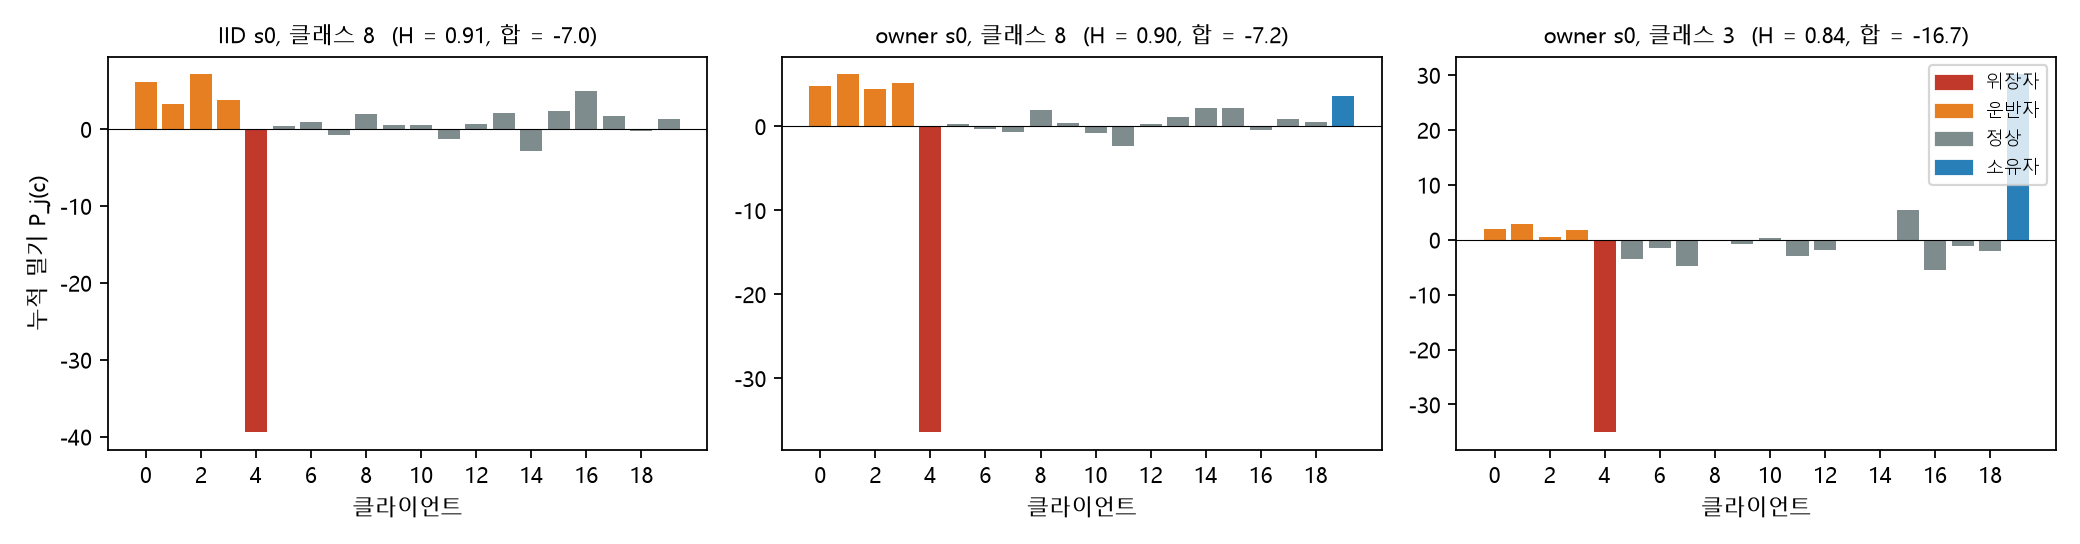
\includegraphics[width=0.49\linewidth]{fig_push_bar.png}\hfill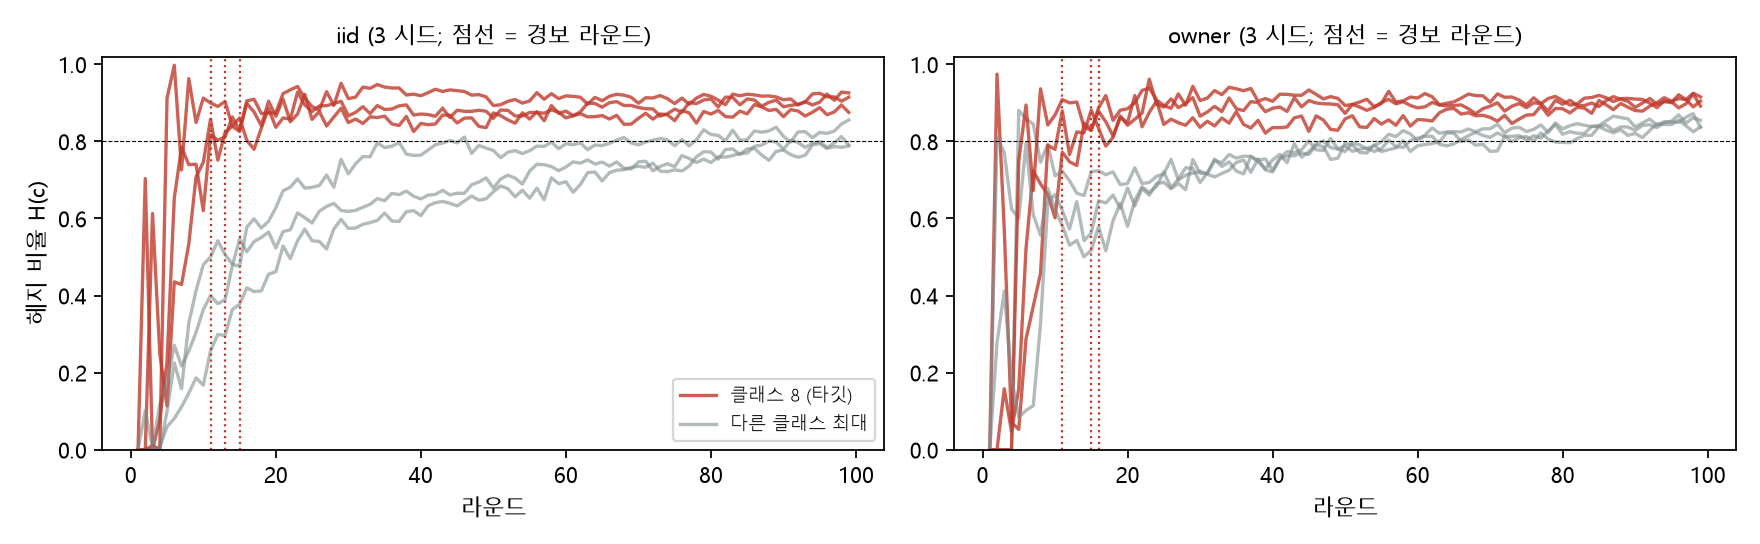
\includegraphics[width=0.49\linewidth]{fig_H_curve.png}\\
{\small 좌: 학습 종료 시 클래스별 누적 기여도(표적 클래스는 주입자 4명이 올리고 억제자 1명이 내림; 소유 클래스는 소유자 1명이 올리고 억제자가 내림). 우: 라운드별 상쇄 지수와 경보 라운드.}

\section{적응형 공격과 다중 공격자: trade-off}
\paragraph{공격자가 움직일 수 있는 것.} (A) 억제 강도 $s$, (B) 주입자 수 $|A|$, (C) 억제자 수 $|S|$, (D) 상쇄의 범위(트리거 영역에만 국한하는가), (E) 공격 강도(트리거 진폭 atk\_eps, 주입 기여의 크기).
\paragraph{(A) 억제 강도.} 보관된 억제자 기여를 $s$배로 줄인 반합성 실험(논문 설정 1 시드, 그림). $s=1$: ASR 7.5, 억제자 $|z|$ 16.5. $s=0.9$: ASR 42.9 (학습 중 이미 드러남), $|z|$ 14.9. $s\le0.7$: 모델 붕괴(정확도 9.8). $|z|<3$이 되는 $s\le0.2$에서는 모델이 쓸모가 없다. 즉 \emph{잠복(낮은 학습 중 ASR)과 탐지 회피(낮은 $|z|$)를 동시에 얻는 $s$는 없다}. 주의: 주입자 학습을 다시 하지 않은 반합성이므로 감도 분석이며, 실제 적응형 공격(억제자 손실 가중치 조정)은 후속 실험이다.\\
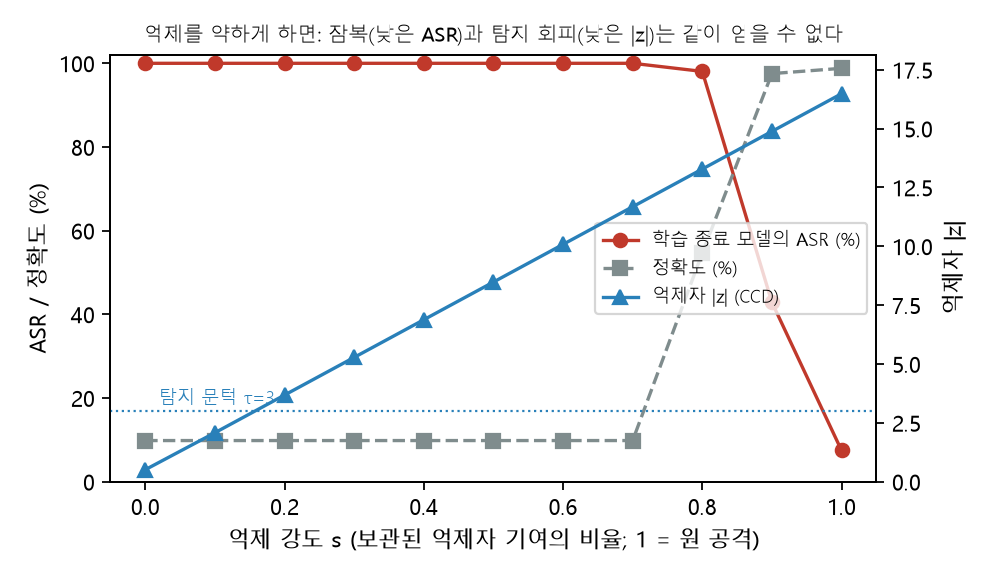
\includegraphics[width=0.62\linewidth]{fig_tradeoff.png}
\paragraph{(B) 주입자 수.} 저자 코드의 \texttt{clients\_ratial}로 주입자 8명·억제자 2명($K=16$) 궤적이 있다. 주입자가 많아져 각자의 기여가 $\kappa$ 아래로 내려가면 $\mathcal{P}$가 비어 주입자 식별은 못 하지만, 총합은 여전히 억제자를 상쇄해야 하므로 $H$와 $z_s$는 남는다(단독 음의 기여로 경보). 즉 공격자는 ``주입자 식별 회피''와 ``주입자당 기여 축소(= 활성화 후 ASR 감소)'' 사이에서 선택한다.
\paragraph{(C) 억제자 수.} 억제를 $n$명에 나누면 각자의 $|z|$가 약 $1/n$로 준다. 음의 기여 집합 규칙 $\mathcal{S}(c)=\{j:z_j\le-\tau\}$로 받으며, $n$이 커질수록 각자가 문턱 아래로 내려가는 대신 활성화에 $n$명 전원의 삭제 요청이 필요해진다(요청 시 층이 $n$번 심사). 억제자 2명 궤적으로 실측 예정.
\paragraph{(D) 상쇄 범위.} 공개 입력에 새지 않게 하면 학습 중 층은 못 본다(BadFU 15 라운드: 경보 없음). 그러나 활성화는 정의상 삭제 대상 입력 위에서 일어나므로 요청 시 층이 받는다(BadFU 로컬: 첫 단계 $z$ 8.4). 두 층이 서로의 경계를 덮는다.
\paragraph{(E) 공격 강도 $\leftrightarrow$ ASR $\leftrightarrow$ 탐지 점수.} 계획: atk\_eps $\in\{0.25,0.5,1\}$, 주입자 수 $\in\{4,8\}$에서 (학습 중 ASR, 삭제 후 ASR, 억제자 $|z|$, 경보 라운드)를 한 표에. 기대: 삭제 후 ASR이 올라갈수록 $|z|$도 단조 증가(둘 다 $|\Phi_S|$에 비례).

\section{발전 방안 (순서)}
\begin{enumerate}
\item \textbf{오탐률.} 공격 없는 궤적(MNIST/CIFAR $\times$ IID/non-IID, 생성 중)에서 경보 0회 실측. 명제 2의 근거.
\item \textbf{규모.} CIFAR-10/ResNet-18 논문 설정 3 시드(생성 중, 1번 궤적 53/100 라운드). 같은 문턱값으로 동작하는지.
\item \textbf{두 번째 공격.} BadFU 40 라운드 3 시드에서 학습 중 층의 경계와 요청 시 층의 보완을 실측.
\item \textbf{적응형.} (A) 억제자 손실 가중치 실제 조정, (B)(C) \texttt{clients\_ratial}=2 궤적, (E) atk\_eps 격자 $\to$ trade-off 표.
\item \textbf{강건 집계 위.} Median·Multi-Krum·FLAME·FLDetector 위 12 궤적에서 두 층.
\item \textbf{이론.} 명제 1·2를 가정(전파 비율 $\eta$, 정상 기여의 독립·산포)과 함께 정리로.
\end{enumerate}
\paragraph{참고.} 자세한 초안: \texttt{docs/paper/draft\_v5.pdf}. 결과 번호: \texttt{docs/RESULTS\_LOG.md}. 실행: \texttt{RUN.md}.
\end{document}
